\documentclass[10pt,aspectratio=169]{beamer}

\usepackage[utf8]{inputenc}
\usepackage[english]{babel}
\usepackage[babel]{csquotes}
\usepackage[T1]{fontenc}
%\usepackage{enumitem}

\usepackage{graphicx}
\usepackage{verbatim}

\usepackage{ae, aecompl}

\setlength {\marginparwidth }{2cm}
\usepackage{todonotes}

\usepackage{array}

\usepackage[backend=biber]{biblatex}
\bibliography{references.bib}

% used for color define
\usepackage{color}
\definecolor{bgsidebar}{rgb}{0,0.1,0.6}
\definecolor{darkgreen}{rgb}{0,0.6,0}
\definecolor{Gray}{gray}{0.5}
\definecolor{highlight}{rgb}{0,0.7,0.5}
\definecolor{lightgray}{gray}{0.5}
\definecolor{lightlightgray}{rgb}{0.83, 0.83, 0.83}
\definecolor{tfblue}{RGB}{0, 61, 134}
\usepackage{xcolor}
\newcommand{\highlight}[1]{\colorbox{lightlightgray}{#1}}

\usepackage{subfigure}

\usepackage{ulem}

\usepackage{textcomp,upquote,lmodern,listings}

\usetheme[sectionpage=none,numbering=fraction]{metropolis}
\setbeamerfont{structure}{shape=\bfseries}
%\usetheme{CAU} 			%Theme
%\usecolortheme{dolphin}
%
%\useoutertheme[left,hideothersubsections,width=20mm,height=0.7cm]{sidebar} % Sidebar links verwenden
%\setbeamertemplate{navigation symbols}{} 
%
%% Breite der Seitenleiste einstellen
%%\setbeamersize{sidebar width left=30mm}
%
%% Breite des Randes zur Sidebar einstellen
\setbeamersize{text margin left=5mm}
%
%\setbeamercolor{section in sidebar}{fg=black,bg=blue!40}
%\setbeamercolor{section in sidebar shaded}{fg=white}
%
%% autoren klein anzeigen
%%\setbeamerfont{author in sidebar}{size=\tiny}
%
%% Überschriften der Folien groß und weiß
%\setbeamerfont{frametitle}{size=\LARGE}
%\setbeamercolor{frametitle}{fg=black}
%\setbeamercolor{frametitle}{bg=white}
%
%\let\oldsection\section
%\renewcommand{\section}[1]{\oldsection[\thesection . #1]{#1}}
%\newcommand{\multilinesection}[2]{\oldsection[\thesection . #1 \hbox{\vbox{\hspace{0.17cm}#2}}]{#1 #2}}
%
%\setbeamertemplate{frametitle}{%
%\begin{beamercolorbox}[ht=0cm,wd=0.9\paperwidth,leftskip=15pt,dp=0ex]{frametitle}
%  \insertframetitle
%\end{beamercolorbox}}

\setbeamertemplate{caption}[numbered]

\setbeamercolor{title separator}{fg=tfblue, bg=tfblue}
\setbeamercolor{background canvas}{bg=white}
\setbeamercolor{frametitle}{bg=tfblue}

% Ggf. auskommentieren, falls kein Inhaltsverzeichnis vor jeder Section
\AtBeginSection{
	\addtocounter{framenumber}{-1}
	\frame{\tableofcontents[currentsection,hideothersubsections]}
}

\title[]{MANVSim: Simulation eines Massenanfalls von Verletzten}
\subtitle[]{Bachelor-Abschlussprojekt/Masterprojekt SoSe 2024}
\author{Jon Stührwoldt, Lukas Voigt, Peter Gausmann, Yannick Illmann, Simon Ohlsen}
\date{27. September 2024}

\begin{document}
\frame{\titlepage}

\begin{frame}{MANV}
	\begin{itemize}
		\item MANV: \alert{Massenanfall von Verletzten}
		\item Begriff aus dem Rettungswesen
		\item Tritt ein bei einem Ereignis mit vielen Verletzten
		\item Probleme:
		      \begin{itemize}
			      \item Koordination der Rettungskräfte
			      \item Verteilung von Ressourcen
			      \item Außergewöhnliche Situation auch für Rettungskräfte
		      \end{itemize}
	\end{itemize}
\end{frame}

\begin{frame}{MANV - Beispiele}
	\begin{examples}
		\begin{figure}
			\begin{center}
				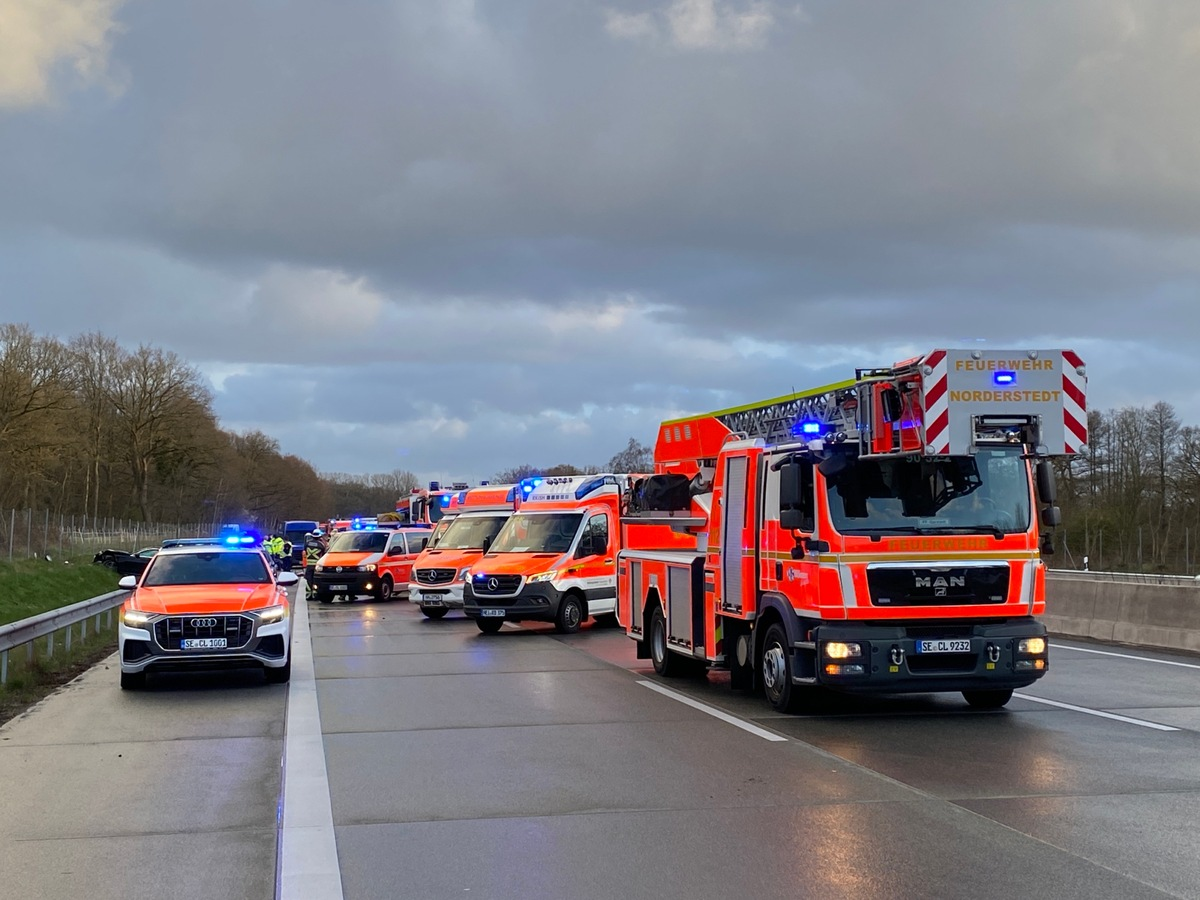
\includegraphics[width=0.4\textwidth]{images/autounfall.jpg}
			\end{center}
			\caption{Autounfall auf A7 zwischen Schnelsen-Nord und Quickborn mit 11 Betroffenen, davon einer tödlich verletzt.\cite{manv-a7}}\label{fig:autounfall}
		\end{figure}
	\end{examples}
\end{frame}

\begin{frame}{MANV - Beispiele}
	\begin{examples}
		\begin{figure}
			\begin{center}
				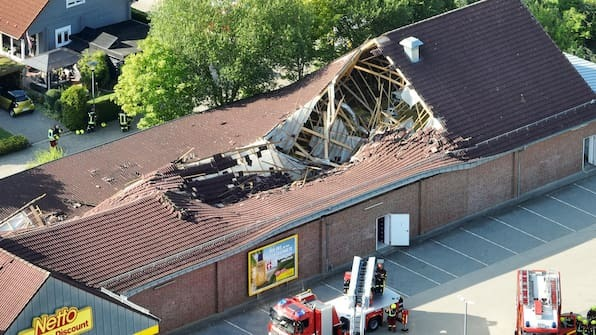
\includegraphics[width=0.5\textwidth]{images/ratzeburg-netto.jpg}
			\end{center}
			\caption{Dacheinsturz eines Supermarktes in Ratzeburg am 30.7.2024. 12 Leichtverletzte.\cite{manv-ratzeburg}}\label{fig:netto}
		\end{figure}
	\end{examples}
\end{frame}

\begin{frame}{MANV - Beispiele}
	\begin{examples}
		\begin{figure}
			\begin{center}
				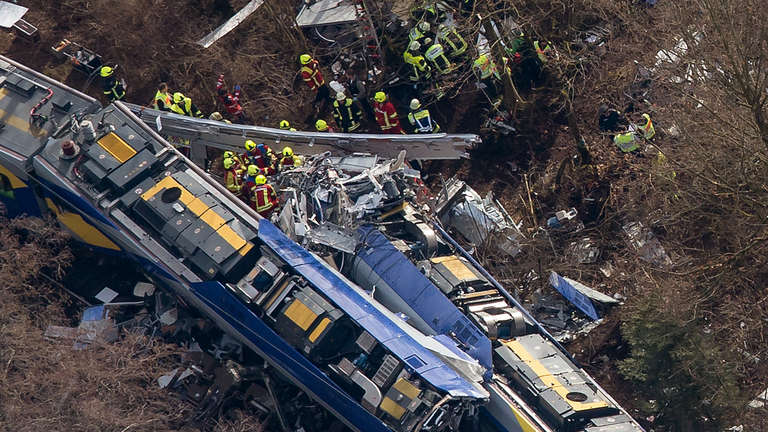
\includegraphics[width=0.5\textwidth]{images/bad-aibling.jpg}
			\end{center}
			\caption{Zugunglück von Bad Aibling. 12 Tote, 18 Schwerverletzte, 63 Leichtverletzte.\cite{manv-badaibling}}\label{fig:badaibling}
		\end{figure}
	\end{examples}
\end{frame}


\begin{frame}{MANV - Übung i}
	\begin{itemize}
		\item Vorbereitung auf den Ernstfall
		\item Regelmäßige Übungen
		\item Nicht standardisiert, jedoch Leitfaden vom DRK \cite{kreuz2016durchfuhrung}
		\item Mögliche Übungsformen:
		      \begin{itemize}
			      \item Von: Übung in Sporthalle mit Blättern als Patienten
			      \item Bis hinzu: Übung mit Mimen, überregionalen Einsatzkräften, Fahrzeugen, Gelände
		      \end{itemize}
		\item Ablauf auf Organisationsebene:
		      \begin{itemize}
			      \item Planung (Szenario, Übungsverlauf, ...)
			      \item Vorbereitung (Termin finden, Mimen anheuern, ...)
			      \item Durchführung
			      \item Direkte Nachbereitung mit allen Beteiligten, direktes Feedback
			      \item Spätere Nachbereitung mit Führungskräften zur Datenauswertung
		      \end{itemize}
	\end{itemize}

\end{frame}

\begin{frame}{MANV - Übung ii}
	\begin{columns}
		\begin{column}{0.7\textwidth}
			\begin{itemize}
				\item Ziel: Teilnehmer sollen lernen, dass\dots
				      \begin{itemize}
					      \item \dots es ein MANV-Konzept gibt und wie es aussieht
					      \item \dots Zeit kostbar ist
					      \item \dots es nicht mehr um individuelle Patientenversorgung geht
					      \item \dots Triage wichtig ist
				      \end{itemize}
			\end{itemize}
		\end{column}
		\begin{column}{0.3\textwidth}
			\begin{figure}
				\begin{center}
					\includegraphics[height=0.4\textheight]{images/übung.jpg}
				\end{center}
				\caption{Übung eines MANV.\cite{manv1übung}}\label{fig:übung}
			\end{figure}
		\end{column}
	\end{columns}
\end{frame}


\section{Simulation}

\begin{frame}{Simulation}
	Anwendung MANVSim
	\begin{itemize}
		\item Webanwendung zur Administration
		\item Mobile App für Übungsteilnehmer
	\end{itemize}
	Unterschiedliche Rechte Gruppen
	\begin{itemize}
		\item Webanwendung:
		\begin{itemize}
			\item Game Master: Leitstelle mit erweiterten Zuständigkeiten
			\item Scenario Manager: Datenmanager + Game Master
			\item Anwendungsadmin: Sicherheitsbeauftragter + Scenario Manager
		\end{itemize}
		\item Übungsteilnehmer: Player 
	\end{itemize}
\end{frame}

\begin{frame}{Anwendung MANVSim - Simulation}
	*Wechsel zur Anwendung*
\end{frame}

%
% Section 3
%
\section{App}

\begin{frame}{App - Kommunikation mit Server}
	Placeholder: Jons Teil
\end{frame}

\begin{frame}{App - Kommunikation mit Server}
	\begin{itemize}
		\item Kommunikation mit Server über REST-API
		\item 19 API Endpunkte
	\end{itemize}
	\centering
	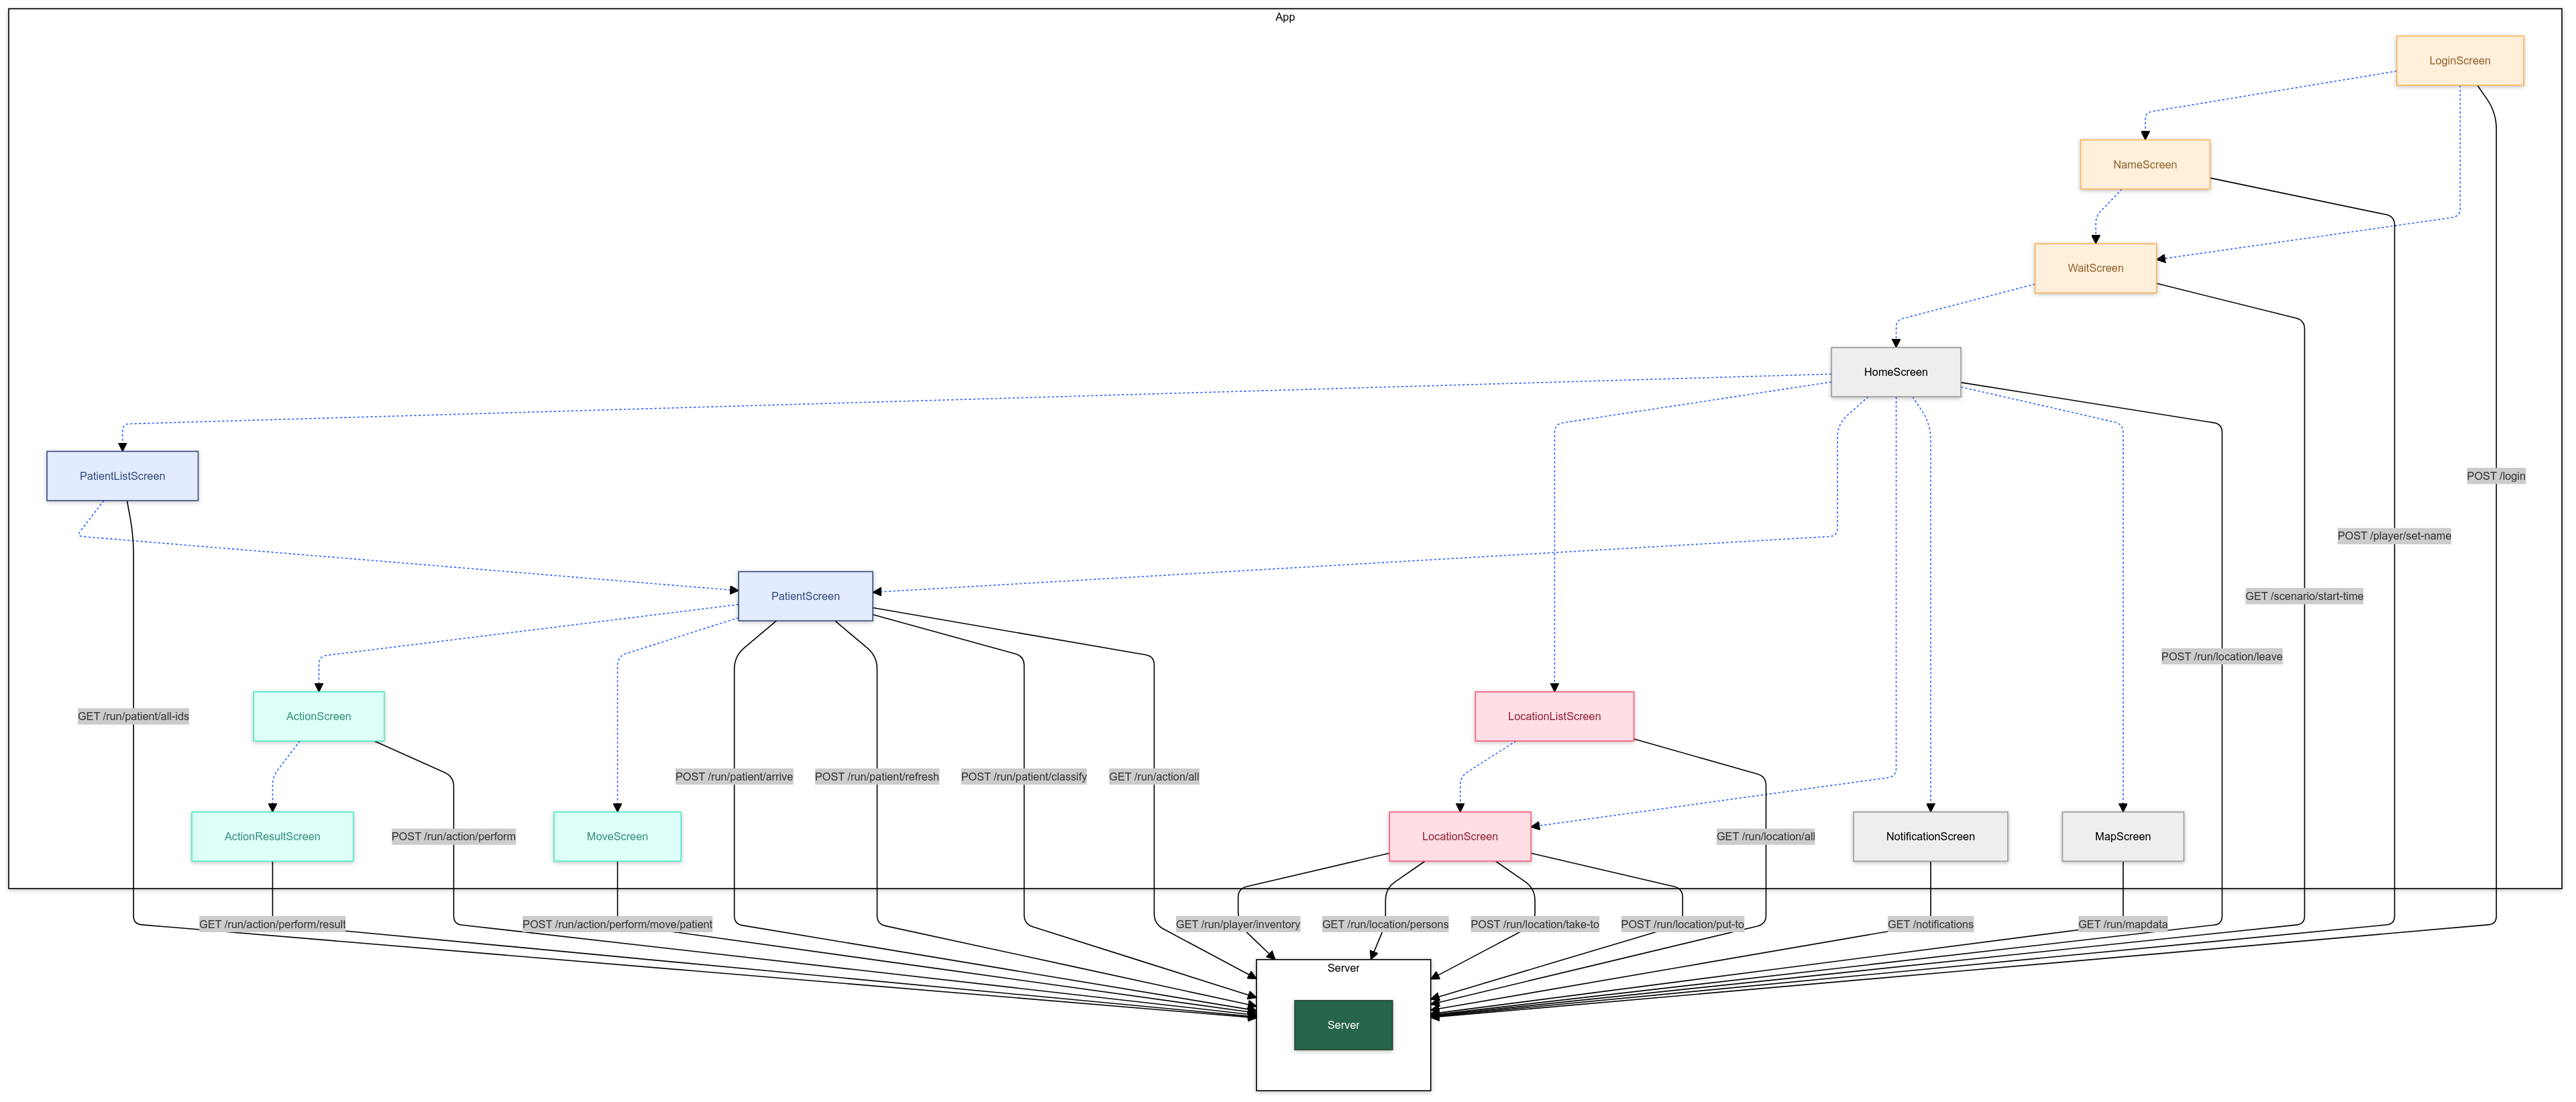
\includegraphics[width=1.0\textwidth]{images/app/server_endpoints.png}
\end{frame}

\begin{frame}{App - Kommunikation mit Server}
	\centering
	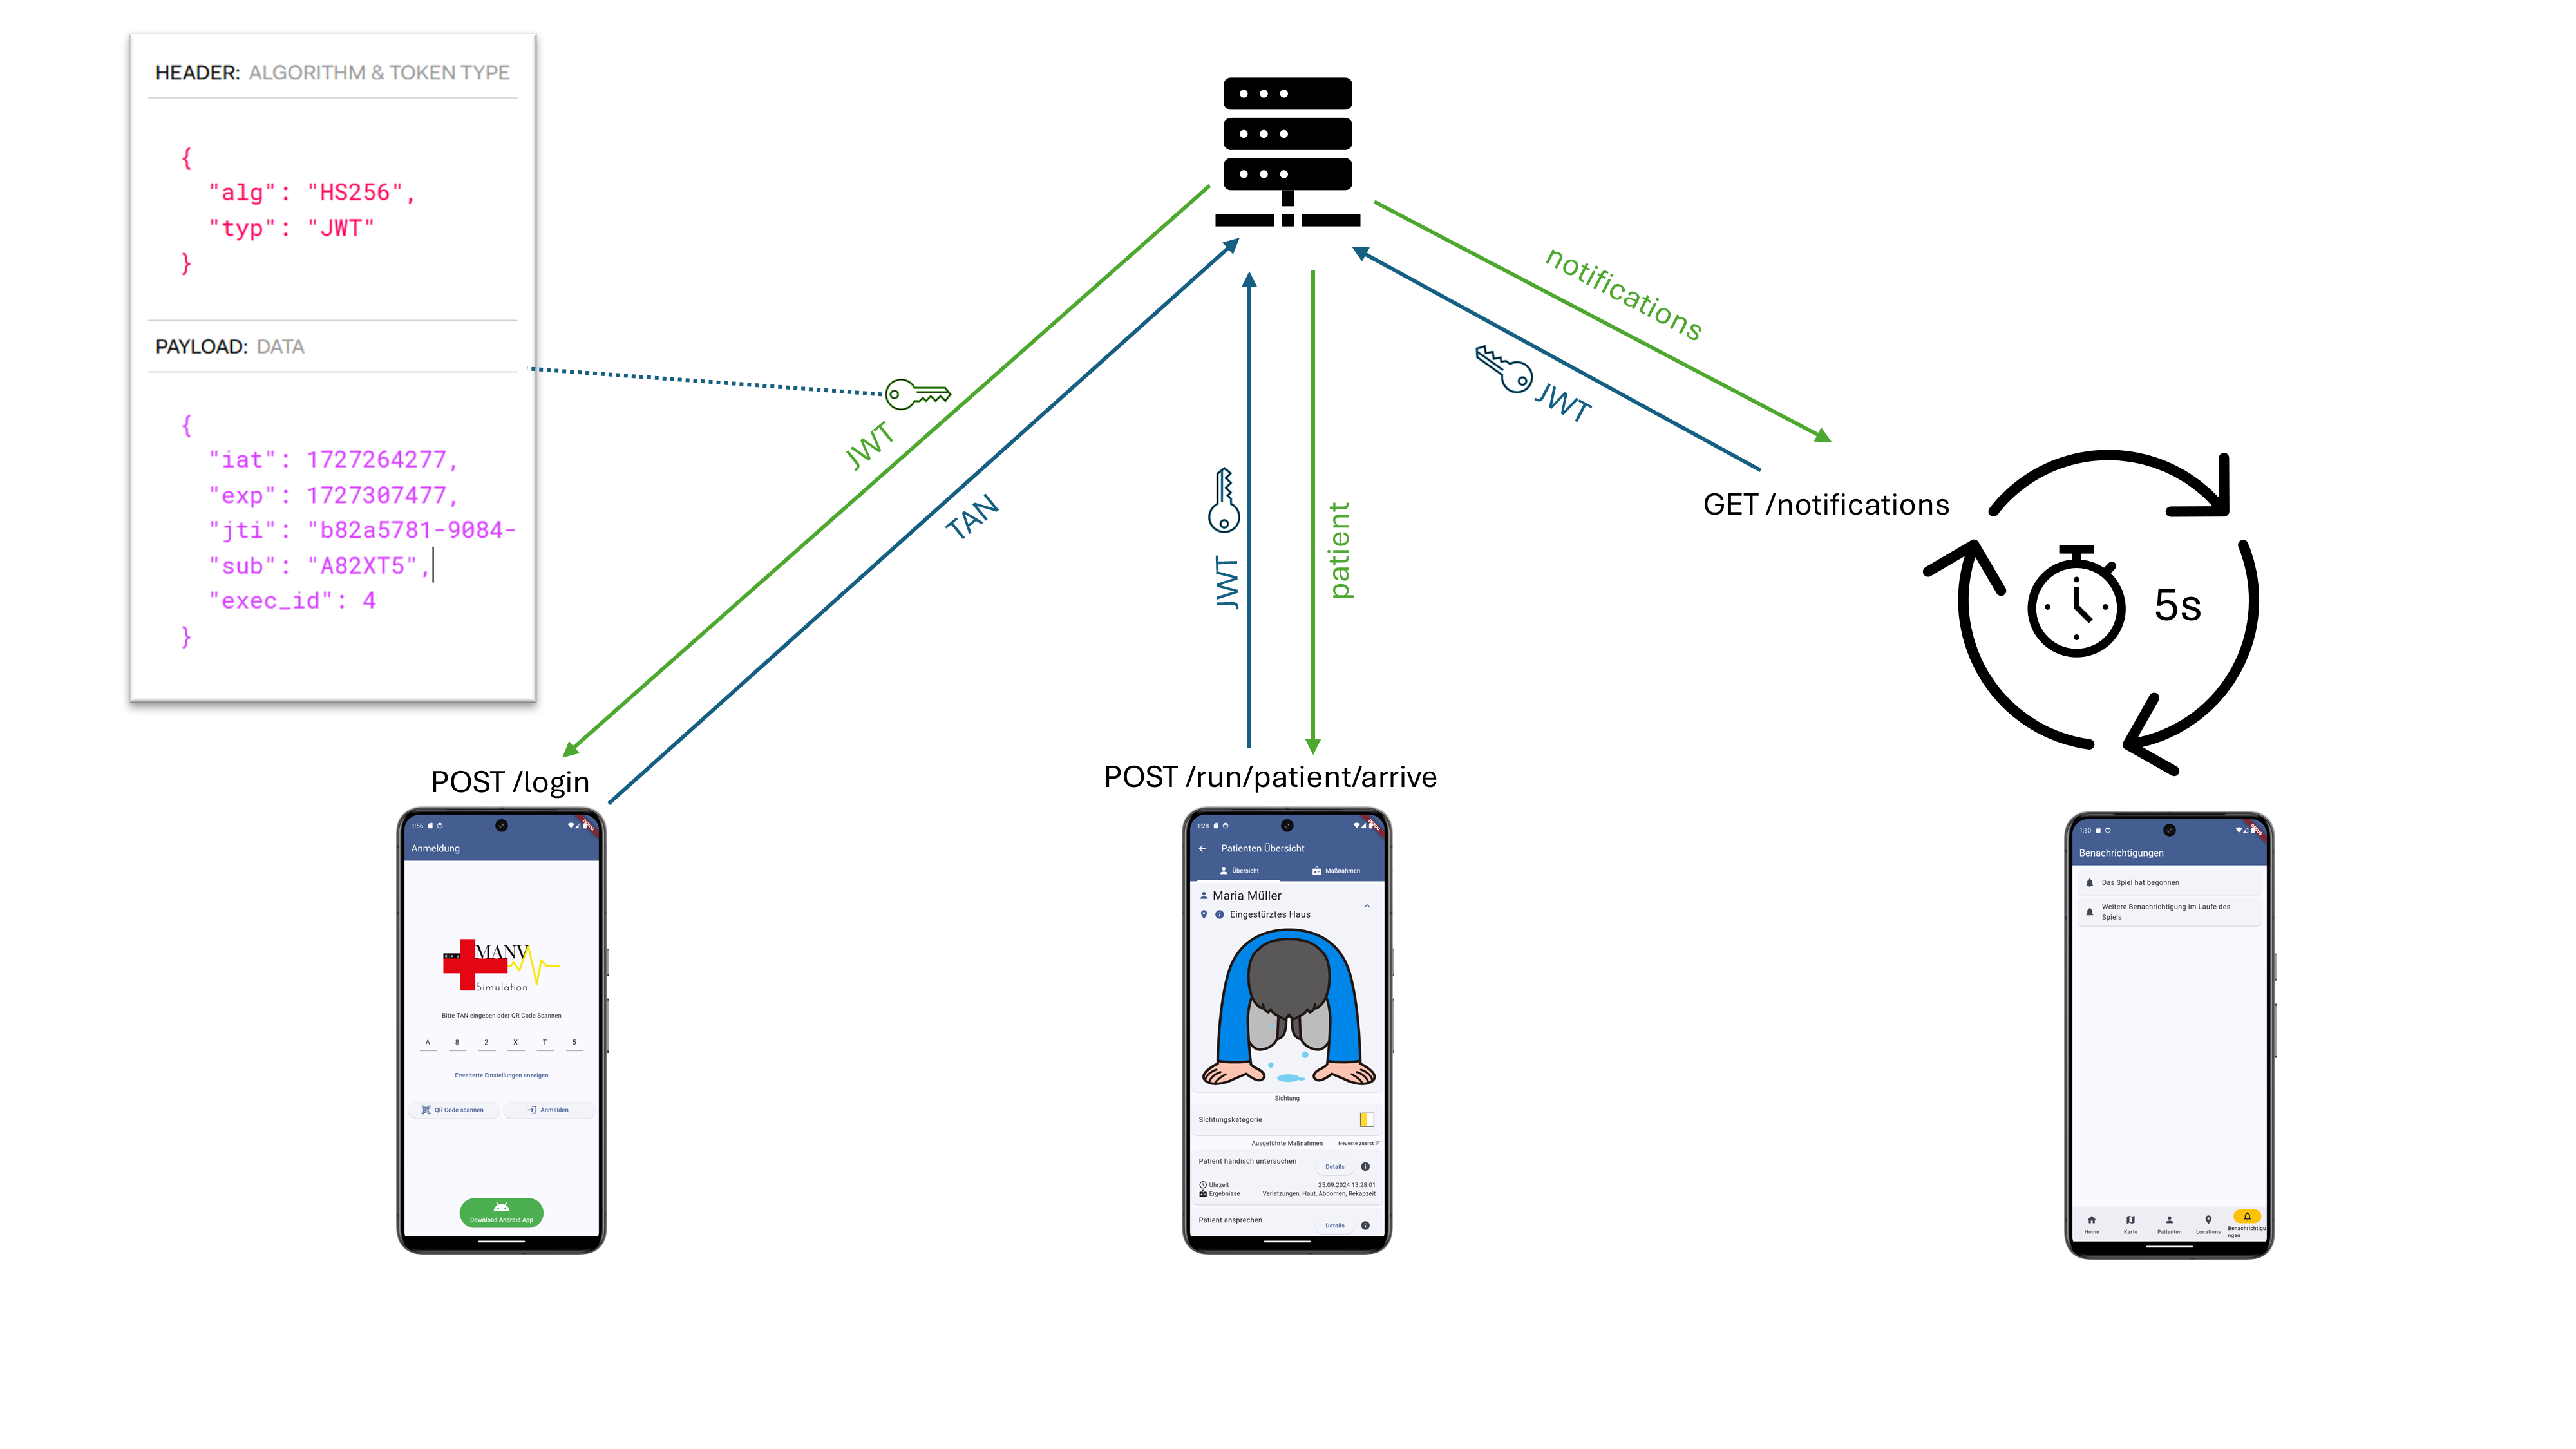
\includegraphics[width=1.0\textwidth]{images/app/api_flow.png}
\end{frame}

\begin{frame}{App - Kommunikation mit Server}
    \vfill
    \begin{figure}
        \centering
        \begin{minipage}{0.3\textwidth}
            \centering
            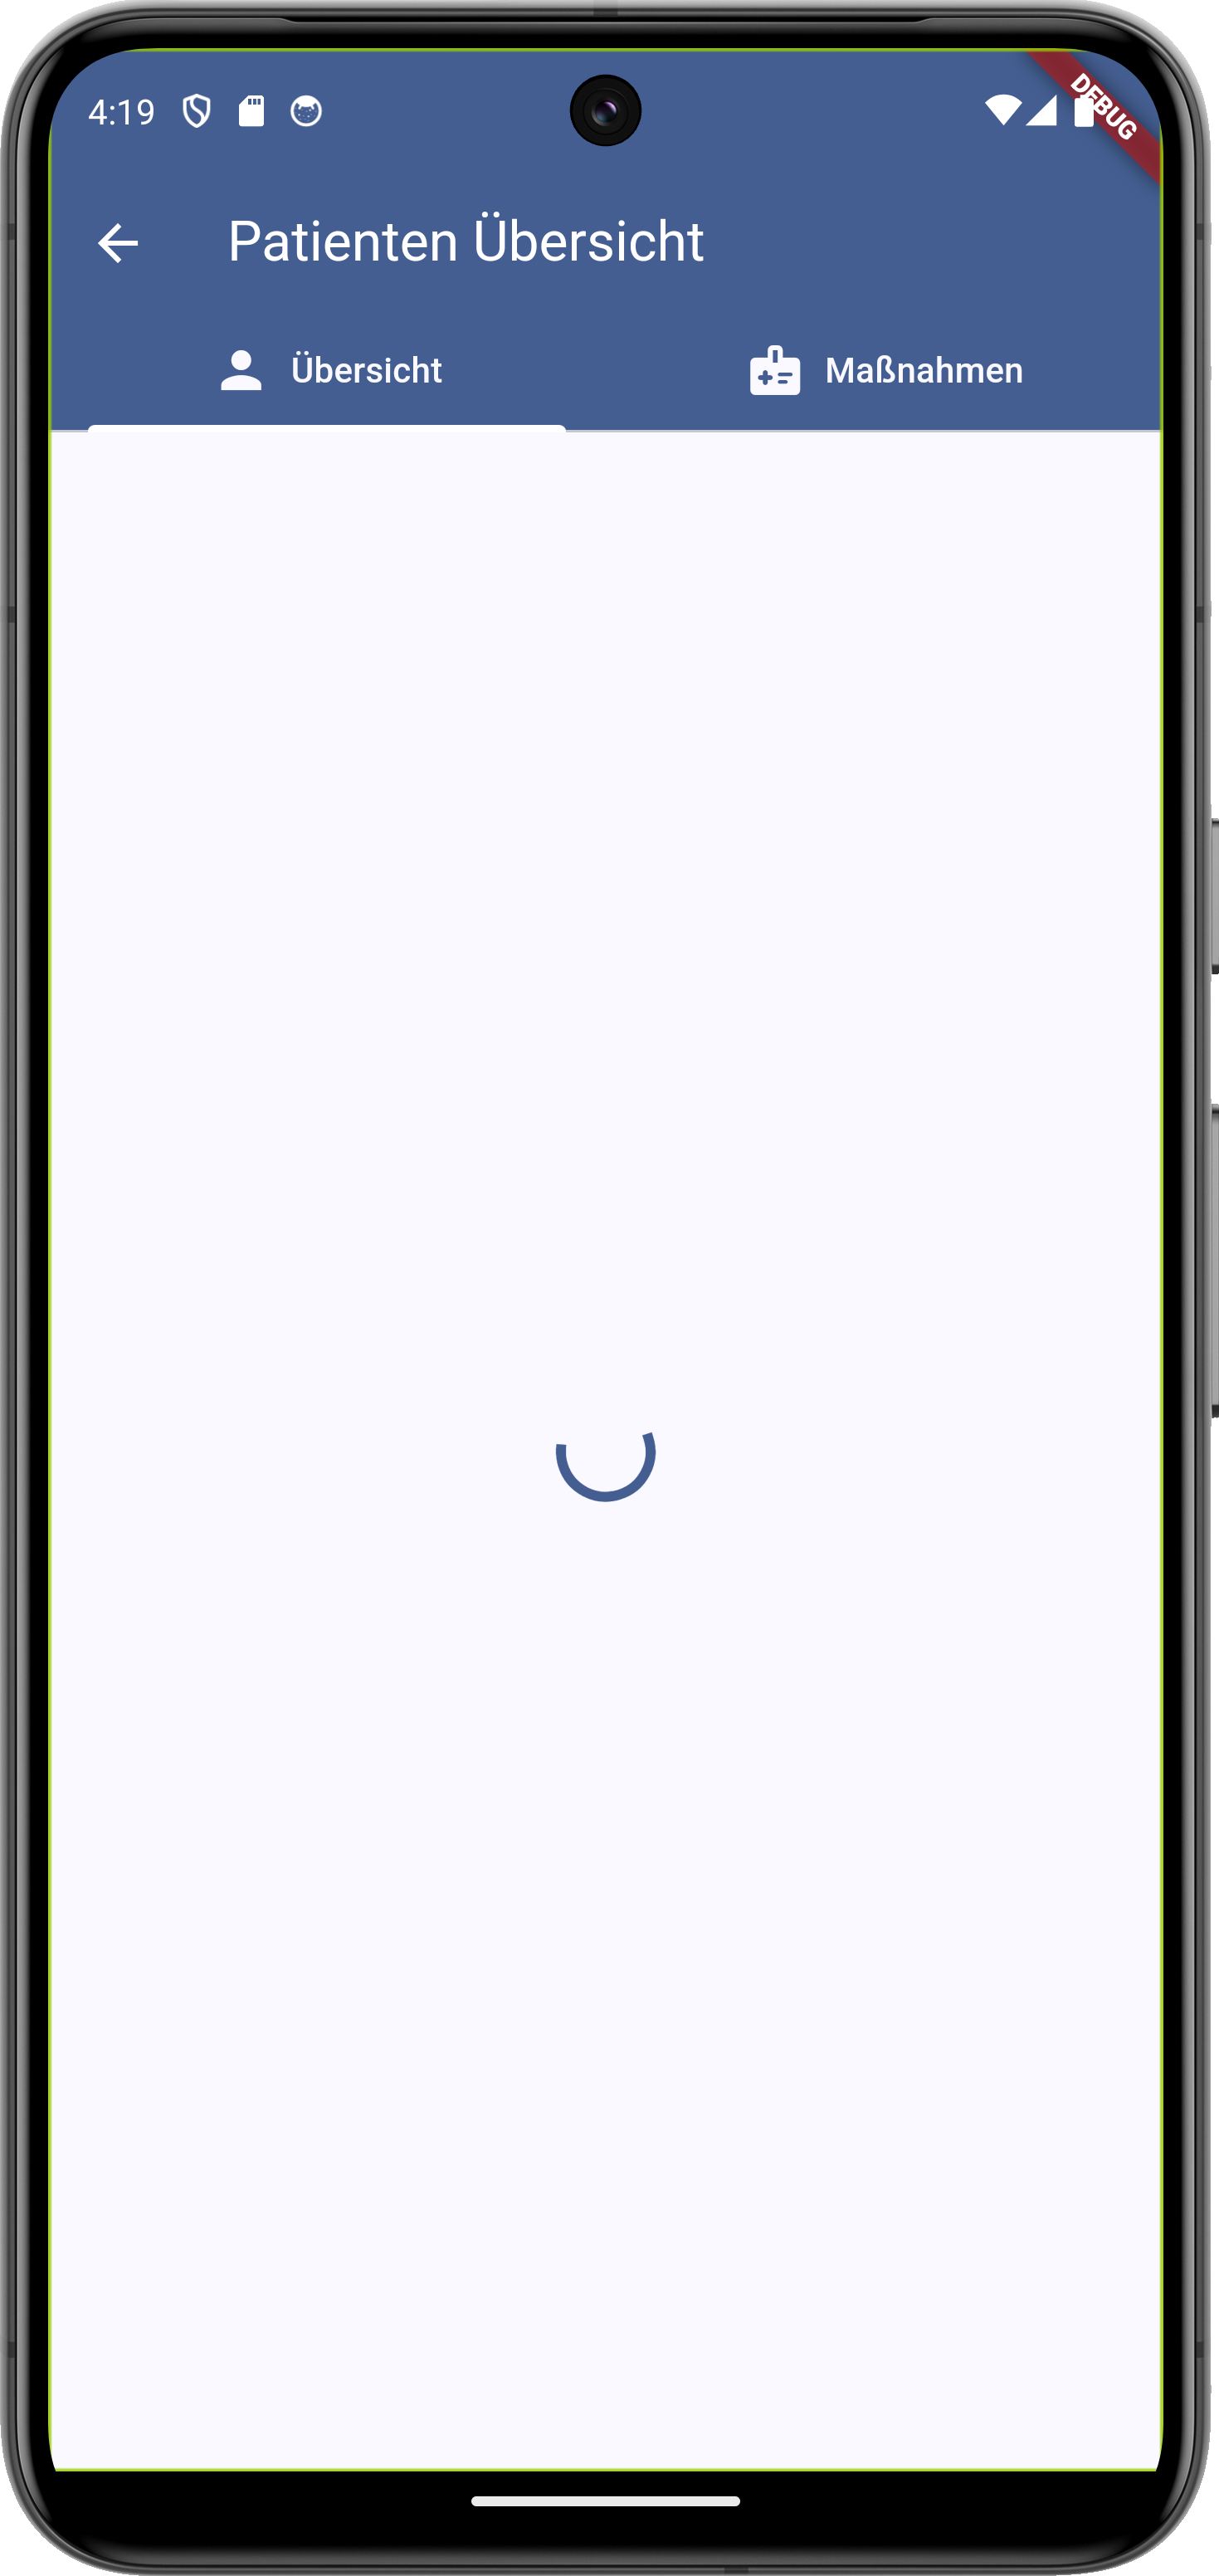
\includegraphics[height=0.8\textheight]{images/app/screenshots/concurrency_loading.png}
            \par{Laden}
        \end{minipage}
        \hspace{0.5cm}
        \begin{minipage}{0.3\textwidth}
            \centering
            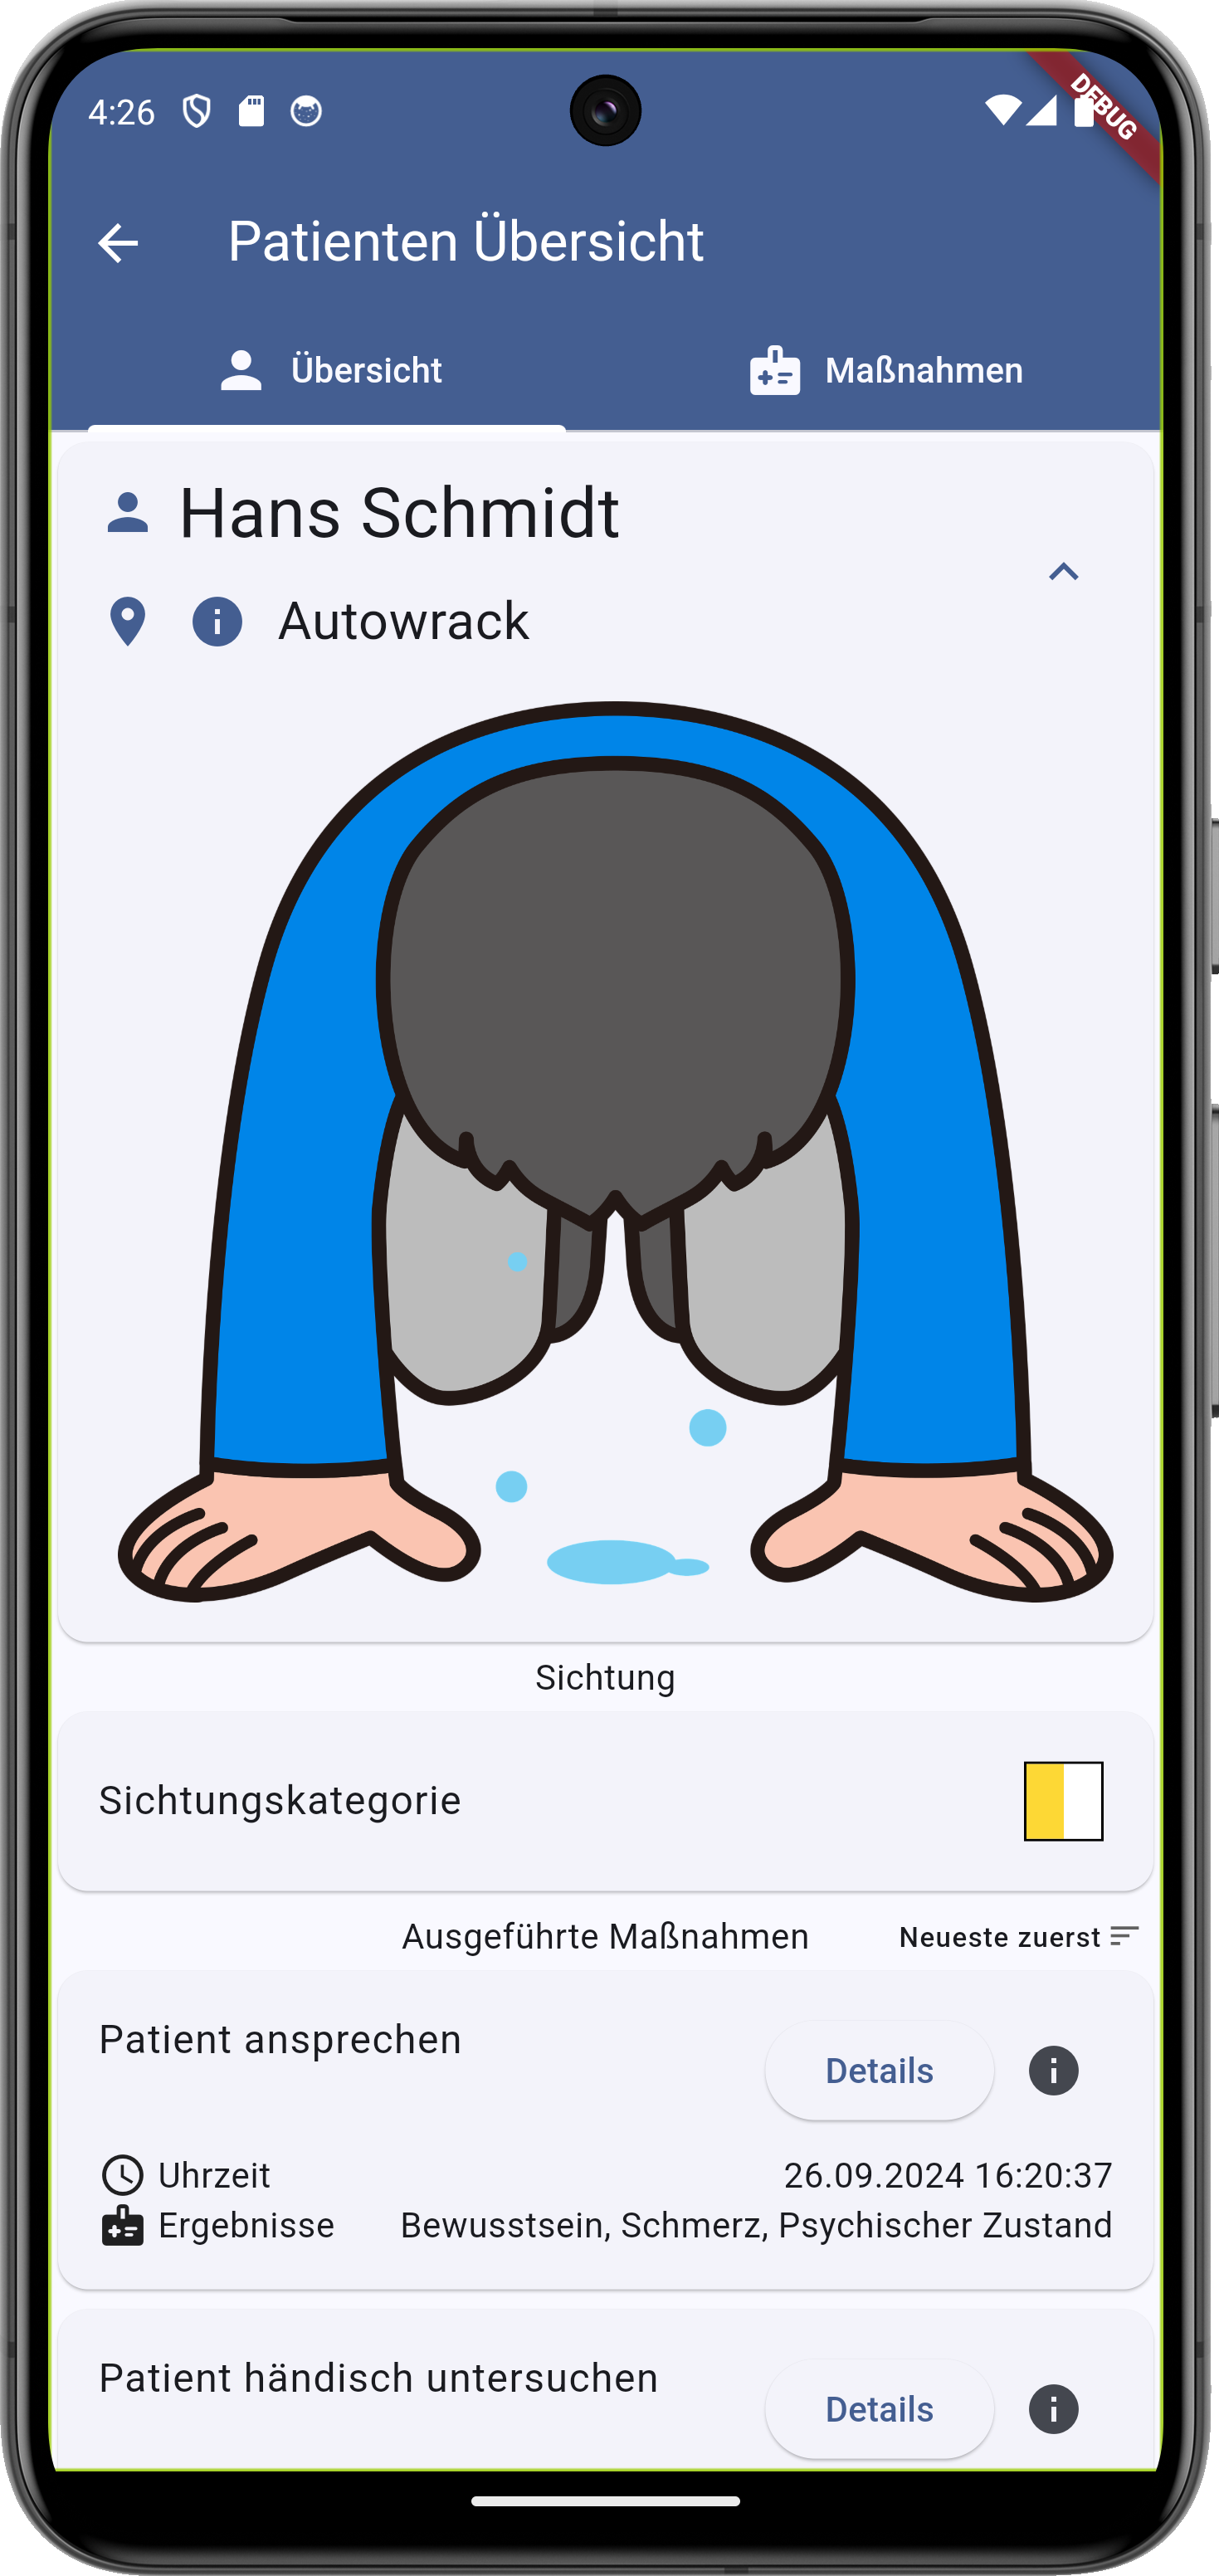
\includegraphics[height=0.8\textheight]{images/app/screenshots/concurrency_ok.png}
            \par{Ereignis}
        \end{minipage}
        \hspace{0.5cm}
        \begin{minipage}{0.3\textwidth}
            \centering
            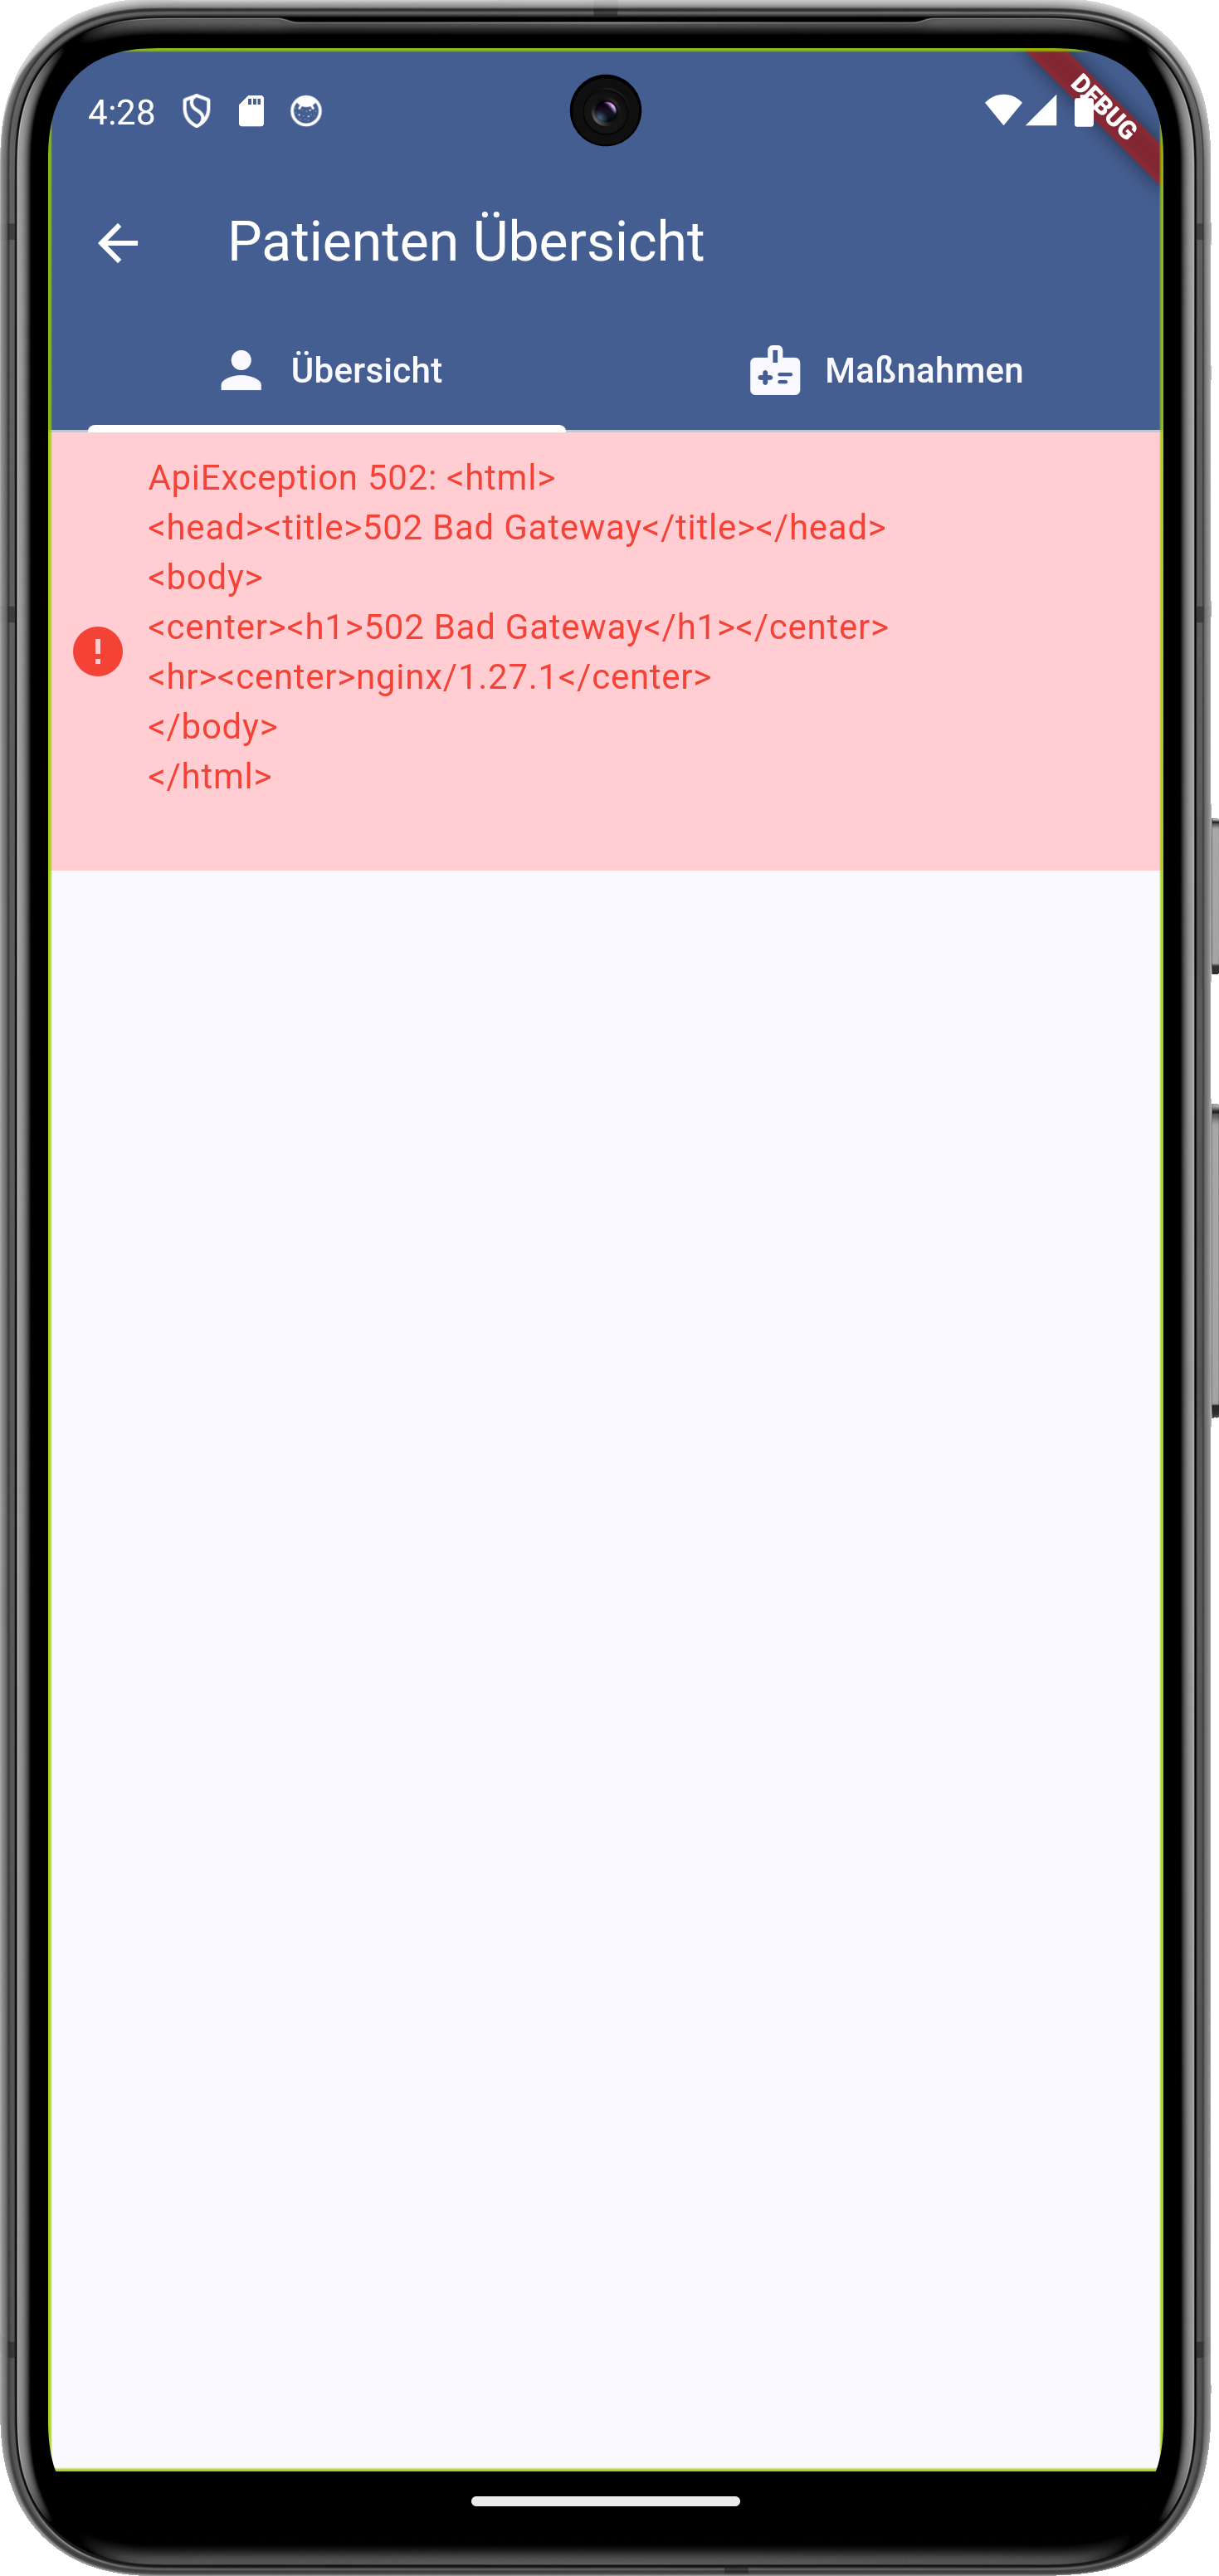
\includegraphics[height=0.8\textheight]{images/app/screenshots/concurrency_error.png}
            \par{Fehler}
        \end{minipage}
    \end{figure}
    \vfill
\end{frame}

\section{Backend}


\begin{frame}{Backend}
	\begin{itemize}
		\item[] Python Server mit Flask API
		\begin{itemize}
			\itemsep 4pt
			\item stellt Endpunkte zum Persistieren der Stammdaten
			\item stellt Endpunkte zur Live Administration einer Übung
			\item stellt Endpunkte zur Teilnahme an einer Übung
		\end{itemize}
	\end{itemize}
\end{frame}


\begin{frame}{Backend-Komponenten}
	\centering
	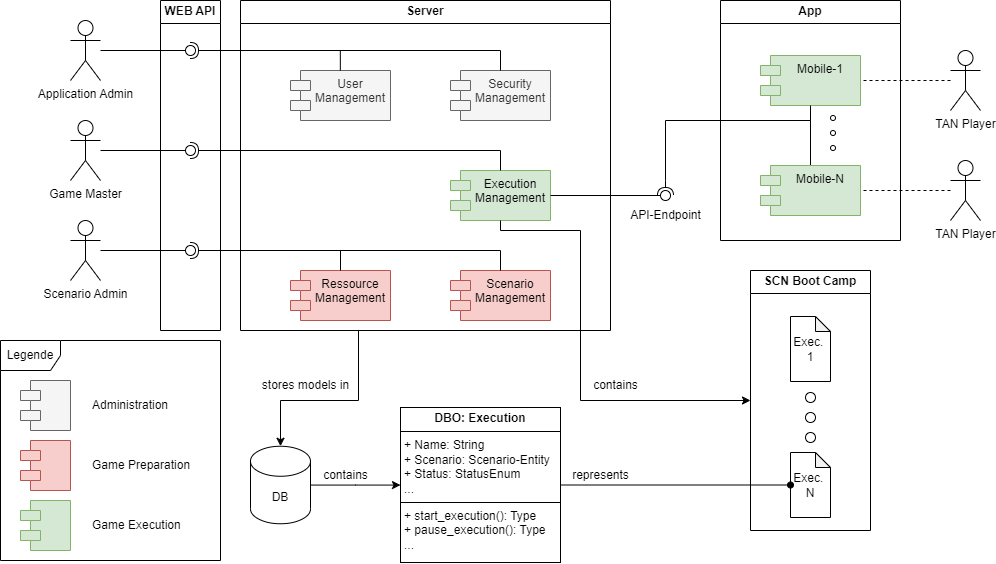
\includegraphics[width=0.7\textwidth]{images/server/component_diagram.png}
\end{frame}


\begin{frame}{Server: Datenhaltung}
	\begin{columns}
		\column{0.7\linewidth}
			\begin{itemize}
				\itemsep 12pt
				\item[] Trennung von Basis- und Spieldaten
				\begin{itemize}
					\itemsep 2pt
					\item[$\rightarrow$] In-memory Objekte für Spieldaten
					\item[$\rightarrow$] Datenbank für Template-Objekte   
				\end{itemize}
				\item[] Vorteile:
				\begin{itemize}
					\itemsep 2pt
					\item Unabhängigkeit von ORM
					\item Konstante schnelle Zugriffszeiten
					\item Kapselung
				\end{itemize}
				\item[] Nachteile:
				\begin{itemize}
					\itemsep 2pt
					\item Erhöhte Komplexität
					\item Synchronisation
				\end{itemize}
			\end{itemize}
		\column{0.3\linewidth}
			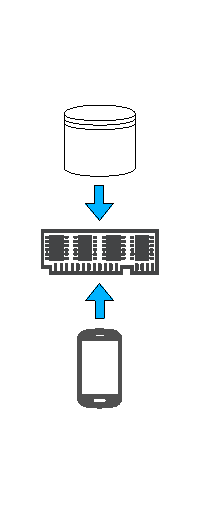
\includegraphics[height=\textheight]{images/server/datenhaltung.pdf}
	\end{columns} 
\end{frame}


\begin{frame}{Server: Laufzeitobjekte}
	\centering
	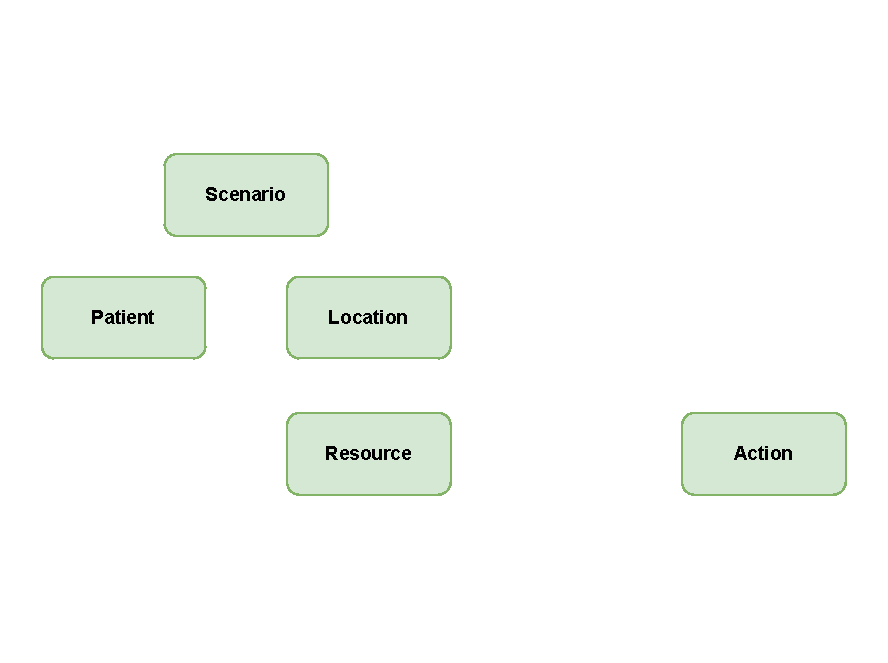
\includegraphics[height=.9\textheight]{images/server/laufzeit_objekte_1.pdf}
\end{frame}

\begin{frame}{Server: Laufzeitobjekte}
	\centering
	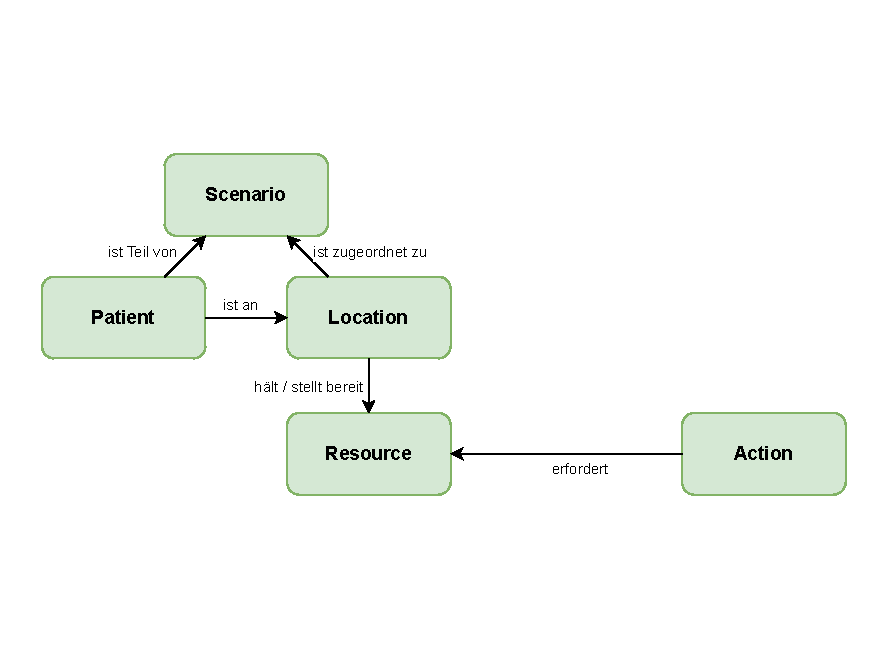
\includegraphics[height=.9\textheight]{images/server/laufzeit_objekte_2.pdf}
\end{frame}

\begin{frame}{Server: Laufzeitobjekte}
	\centering
	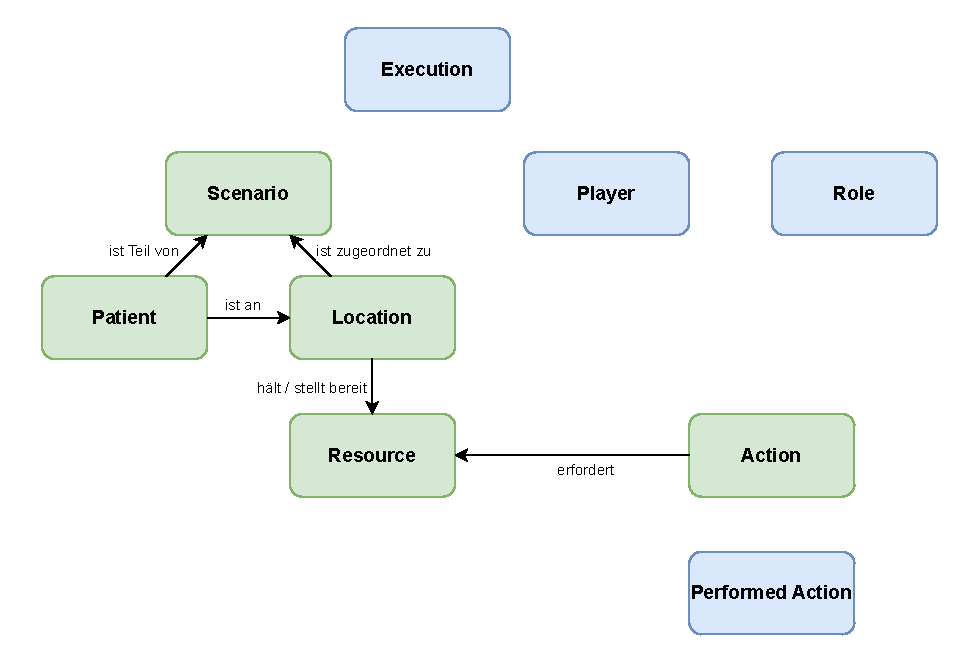
\includegraphics[height=.9\textheight]{images/server/laufzeit_objekte_3.pdf}
\end{frame}

\begin{frame}{Server: Laufzeitobjekte}
	\centering
	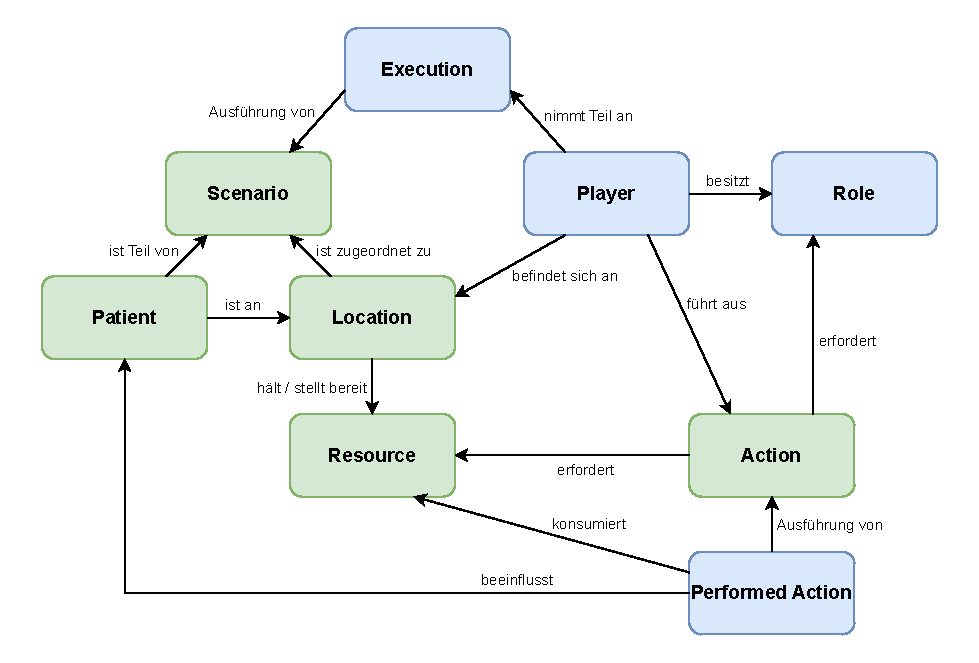
\includegraphics[height=.9\textheight]{images/server/laufzeit_objekte.pdf}
\end{frame}


\begin{frame}{Server: Datenbankobjekte}
	\centering
	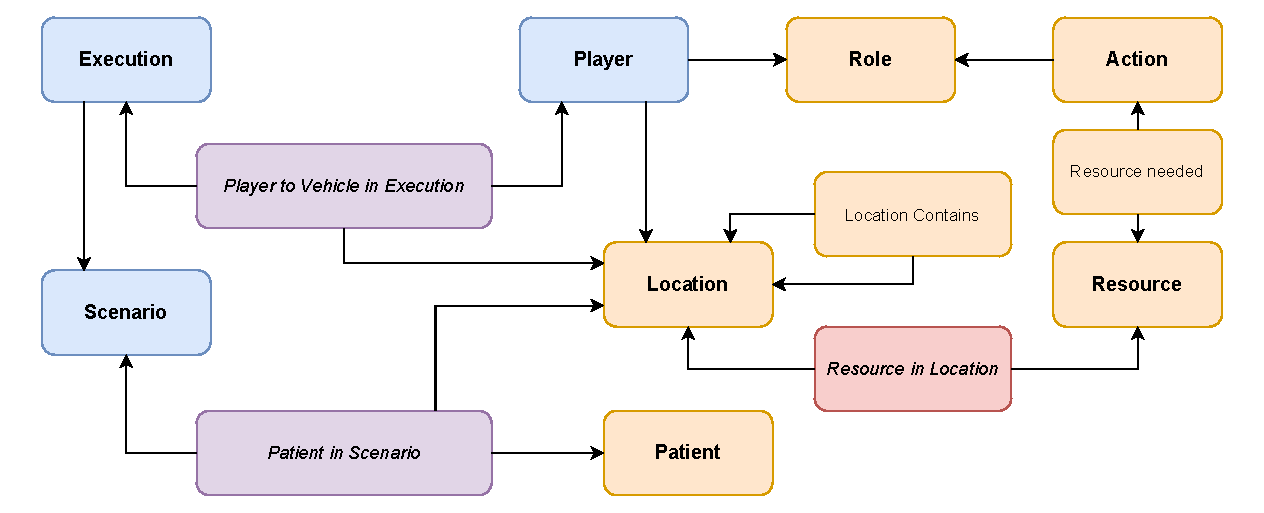
\includegraphics[width=\textwidth]{images/server/datenbank_objekte.pdf}
\end{frame}

\section{Projektarbeit Evaluation}

\begin{frame}{Rückblick}
	Projektarbeit MANVSim 
	\begin{itemize}
		\item Weekly Termin mit ergänzenden Einzelterminen
		\item Feature-Branch Implementierung
		\item Review Prozesse für gemeinsamen Wissensaustausch
	\end{itemize}
    Herausforderungen
	\begin{itemize}
		\item Unterschiedliches KnowHow vereinen
		\item Mehrere Entwicklungsschwerpunkte (Web, Python, Mobile)
		\item Stundenpläne und (Krank-)Ausfälle ändern Prioritäten
	\end{itemize}
\end{frame}
\begin{frame}{Ausblick}
	Future Work - Webanwendung
	\begin{itemize}
		\item Erweiterung/Optimieren der Admin-Oberflächen
		\item Neustarten von Übungen basierend auf LogEvents
		\item Statistische Auswertung
		\item User-Management Komponente + Rollen/Rechte erweitern 	
	\end{itemize}

    Future Work - Mobile App / GameAPI
	\begin{itemize}
		\item Resourcen in Inventar Management integrieren
		\item Verbessertes Monitoring der Teilnehmer
		\item Teilnehmer über Hinweise anleiten
		\item IOS Deployment optimieren
	\end{itemize}
\end{frame}

%
% Refs
%

\begin{frame}{Referenzen}
	\printbibliography
\end{frame}

\end{document}
